\section{Resultats}
\captionsetup[figure]{labelsep=space}
\subsection{Descripció de les dades}


\subsection{Anàlisi}
\subsubsection{Comparació de l'ocupació d'aules on hi ha classe amb aules on no n'hi ha}
L'objectiu d'aquest apartat és comparar el percentatge d'ocupació d'ordinadors en les aules on es fa classe i les aules on no se n'hi fa.

Com a premisses fem les següents suposicions:
\begin{enumerate}
	\item Les variables aleatòries \emph{X} i \emph{Y} es poden aproximar a una normal degut a la seva grandària (11934 i 11951, respectivament).
	\item Les diverses mostres preses de \emph{X} i \emph{Y} són consecutives i per tant no independents. Tanmateix, sí que podem suposar que al cap d'una hora d'haver pres una mostra, la nova mostra ja serà independent de l'anterior (suposem que hi ha prou moviment a les aules). Així doncs, si agaféssim només una de cada 60 mostres (1 cada hora), tindríem poblacions mostrals de, aproximadament, 200 individus, que són prou grans com per poder dir que \emph{X} i \emph{Y} s'aproximen a una normal (vegeu figures 1 i 2).
\end{enumerate}

\begin{figure}[h!]
\begin{minipage}{0.5\linewidth}
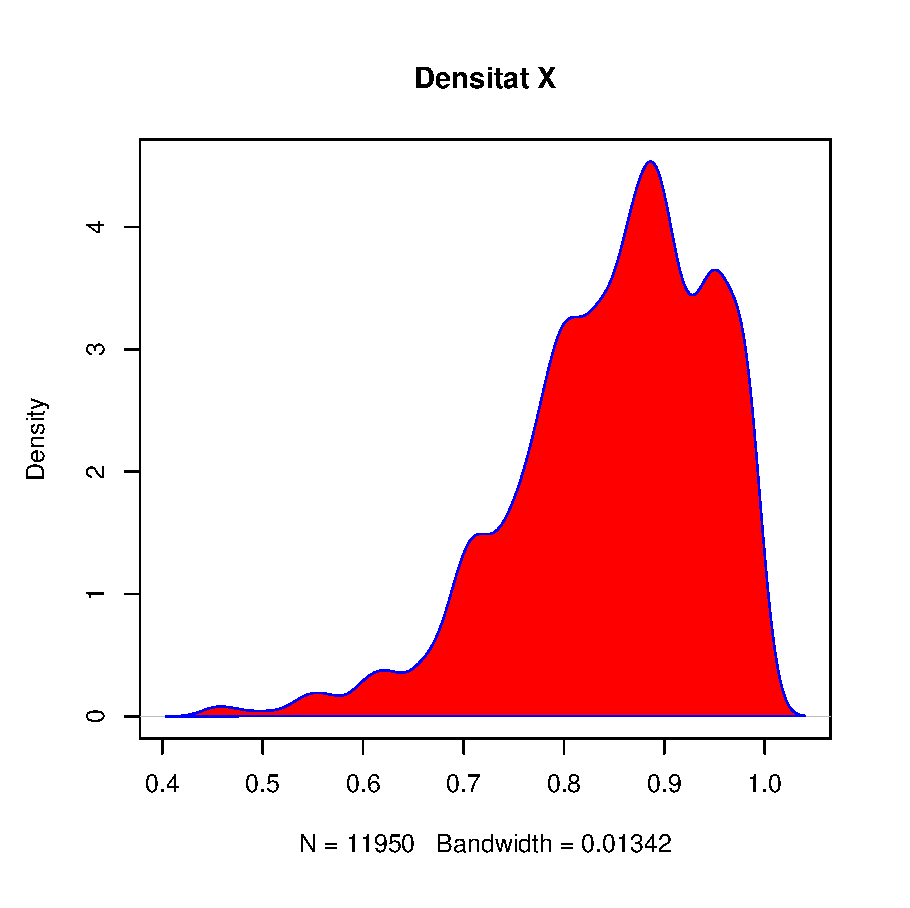
\includegraphics[width=1\linewidth]{./images/no_DENS.eps}
\caption{}
\end{minipage}
\hfill
\begin{minipage}{0.5\linewidth}
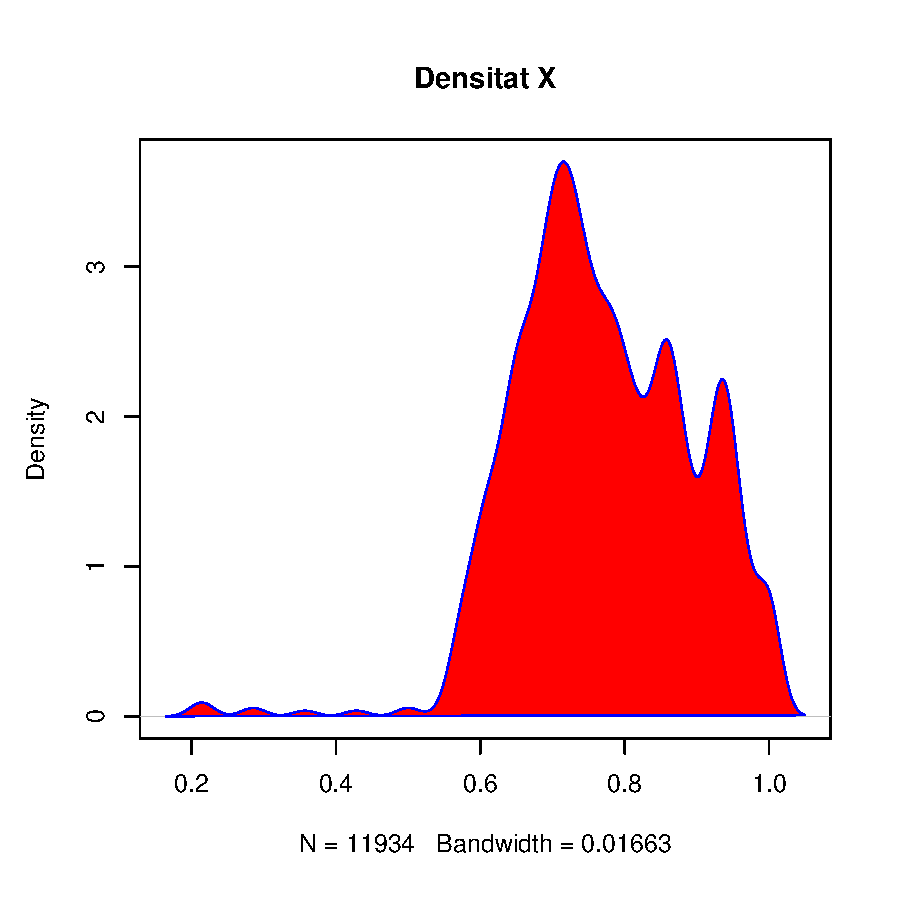
\includegraphics[width=1\linewidth]{./images/si_DENS.eps}
\caption{}
\end{minipage}
\end{figure}

Contrast d'hipòtesis:
$$H0: \mu_x = \mu_y$$
$$H1: \mu_x \neq \mu_y$$

Estadístic utilitzat:
$$\hat{z} = \frac{\bar{x} - \bar{y}}{\sqrt{s_x^2/n_x + s_y^2/n_y}} $$
on: \\
$\bar{x} = 0.77083$,
$s^2_x = 0.01459139$,
$n_x = 11934$ \\
$\bar{y} = 0.8503347$,
$s^2_y = 0.009507904$,
$n_y = 11950$
\\

I per tant:
$$\hat{z} = -55.96263$$
El valor de $\hat{z}$ és extremament petit. De fet, calculant el p-valor amb \emph{R} per aquesta $\hat{z}$ el resultat és 0. Per tant, queda clar que s'ha de rebutjar la hipòtesi nul·la. És més, degut a que $\hat{z}$ ha resultat ser negativa, podem afirmar que $Y>X$.

\subsubsection{title}
